\chapter{Mixer Page:}
The mixer page graphically illustrates the Volume Levels of the sixteen MD tracks of the current Kit.\\
\\
The trigger interface is used in conjunction with \textbf{[ Encoder 1]} to raise or lower the volume of multiple tracks simultaneously. The remaining encoders can be used to adjust the filter parameters of the selected tracks. \\
\\
\fbox{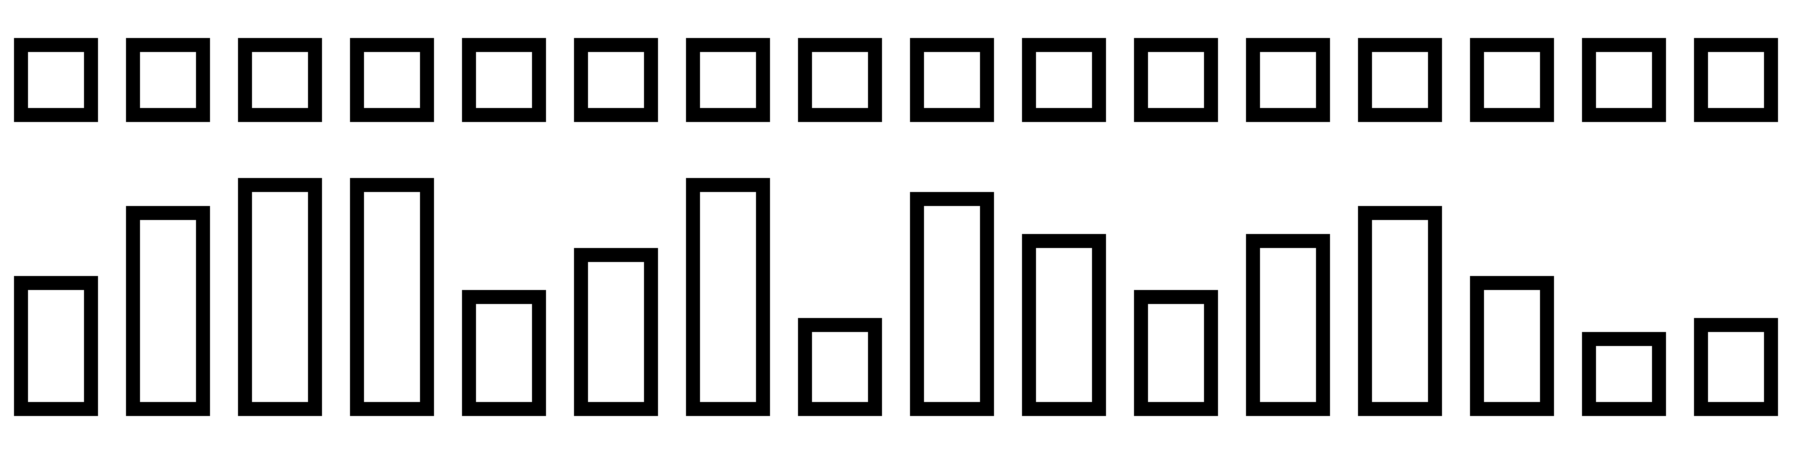
\includegraphics[scale=.40]{mixer_page_init.png}}\\\\
\textit{The Mixer Page is accessible from the PageSelect page.}
\section{Encoder Assignment:}
\begin{itemize}
	\item \textbf{[ Encoder 1 ]: } Level
	\item \textbf{[ Encoder 2 ]: } FLTF (Filter Frequency)
    \item \textbf{[ Encoder 3 ]: } FLTW (Filter width)
	\item \textbf{[ Encoder 4 ]: } FLTQ (Filter resonance)
\end{itemize}


\section{Audio Mutes}
The top row of mixer page shows the Audio Mute state of each Track. \\
This should not be confused with the the MD's sequencer mute state. \\The audio mute state changes the audio routing of muted tracks. When a track is muted from the Mixer Page, audio is routed to the Audio Output specified on the Route Page.
\\
Holding down \textbf{[ Chain ]} and pressing a trigger button on the MD allows you to quickly toggle the mute state of a track.\\
\section{Audio Solo}
Holding down \textbf{[ Save ]} and pressing a trigger button on the MD allows you to quickly solo selected tracks.
